%%%%%%%%%%%%%%%%%%%%%%%%%%%%%%%%%%%%%%%%%%%%%%%%%%%%%%%%%%%%%%%%%%%%%%
%% newminsetpresentation.tex
%% PhD Defence — From Scratch
%% Synthesised from: chapterconflict.tex, conflictmeat.tex,
%%   chaptercontract.tex, forwardtight.tex, forwardlooking2.tex,
%%   quantitativeviol.tex, qviol.tex
%%%%%%%%%%%%%%%%%%%%%%%%%%%%%%%%%%%%%%%%%%%%%%%%%%%%%%%%%%%%%%%%%%%%%%
\documentclass[9pt,aspectratio=169]{beamer}

\usepackage[T1]{fontenc}
\usepackage[utf8]{inputenc}
\usepackage[english]{babel}
\usepackage{amsmath,amssymb,mathtools}
\usepackage{stmaryrd}
\usepackage{xspace}
\usepackage{tikz}
\usetikzlibrary{arrows.meta,positioning,calc,fit,backgrounds,
  decorations.pathreplacing,patterns,shapes.geometric,automata}
\usepackage{bm}

\usetheme{HLISP}

% ── Colour palette ────────────────────────────────────────────────
\definecolor{ConflictBlue}{RGB}{17,84,124}
\definecolor{ConflictGreen}{RGB}{43,122,83}
\definecolor{ConflictRed}{RGB}{178,53,52}
\definecolor{ConflictOrange}{RGB}{215,137,34}
\definecolor{ConflictGray}{RGB}{70,70,70}
\definecolor{SoftBlue}{RGB}{230,240,247}
\definecolor{SoftGreen}{RGB}{232,244,236}
\definecolor{SoftRed}{RGB}{248,233,232}
\definecolor{SoftOrange}{RGB}{250,240,226}

% ── Notation macros (self-contained, no \input{macros}) ───────────
\newcommand{\logic}[1]{\ensuremath{\mathsf{#1}}\xspace}
\newcommand{\TDDLfm}{\logic{\mu MTNL}}
\newcommand{\cDL}{\logic{TACNL}}
\newcommand{\Prog}{\ensuremath{\mathsf{Prog}}\xspace}
\newcommand{\repair}{\ensuremath{\blacktriangleright}}
\newcommand{\obl}[2][]{\mathbf{O}_{#1}(#2)}
\newcommand{\frb}[2][]{\mathbf{F}_{#1}(#2)}
\newcommand{\perm}[2][]{\mathbf{P}_{#1}(#2)}
\newcommand{\repit}[1]{\mathbf{Rep}(#1)}
\newcommand{\guard}[2][]{\lceil #1 \rceil #2}
\newcommand{\trig}[2][]{\langle\!\langle #1 \rangle\!\rangle #2}
\newcommand{\trace}[1]{\ensuremath{\langle #1 \rangle}\xspace}
\newcommand{\emptytrace}{\ensuremath{\trace{-}}}
\newcommand{\emptc}{\ensuremath{\epsilon_{C}}}
\newcommand{\nd}{\text{ and }}
\newcommand{\sor}{\text{ or }}
\newcommand{\is}{\ensuremath{\mathfrak{I}}}
\newcommand{\dpnf}{\ensuremath{\mathsf{DPNF}}}
\newcommand{\pnf}{\ensuremath{\mathsf{PNF}}}
\newcommand{\dnf}{\ensuremath{\mathsf{DNF}}}
\newcommand{\cd}{\ensuremath{\mathsf{C_\delta}}\xspace}
\newcommand{\Namb}{\ensuremath{\mathsf{CFR}}\xspace}
\newcommand{\pt}{\ensuremath{\mathsf{pt}}}
\newcommand{\mathcall}[1]{\text{\usefont{OMS}{cmsy}{m}{n}#1}}
\newcommand{\size}[1]{\vert #1\vert}
\newcommand{\LUCO}{\ensuremath{\mathrm{LUCO}}\xspace}
\newcommand{\LAP}{\ensuremath{\mathrm{LAP}}\xspace}
% Tight verdicts
\newcommand{\topt}{\top^t}
\newcommand{\bott}{\bot^t}
\newcommand{\topp}{\top^p}
\newcommand{\botp}{\bot^p}
\newcommand{\bottp}[1]{\mathbin{\bot^{t}_{#1}}}
\newcommand{\botpp}[1]{\mathbin{\bot^{p}_{#1}}}
% Semantic brackets
\newcommand{\satt}{\models_{\topt}}
\newcommand{\violt}{\models_{\bott}}
\newcommand{\presat}{\models_{?}}
\newcommand{\postsat}{\models_{\topp}}
\newcommand{\postviol}{\models_{\botp}}
\newcommand{\tightverdicts}{\ensuremath{\mathbb{V}_5}\xspace}
% Quantitative
\newcommand{\qsem}[1]{\llbracket #1 \rrbracket_{\text{qviol}}}
\newcommand{\qblame}[1]{\llbracket #1 \rrbracket_{\text{qblame}}}
\newcommand{\qscore}{\ensuremath{\mathsf{Score}}}
\newcommand{\qmc}{\ensuremath{\mathsf{QMC}}}
\newcommand{\qbm}{\ensuremath{\mathsf{QBM}}}
\newcommand{\LH}{\ensuremath{\mathsf{LH}}}
\newcommand{\bmc}{\ensuremath{\mathsf{BMC}}}
\newcommand{\tsmc}{\ensuremath{\mathsf{TSMC}}}
\newcommand{\rrcs}[1]{\ensuremath{\mathsf{RRC}\!\left(#1\right)}\xspace}
\newcommand{\CPM}{\ensuremath{\mathsf{CPM}}\xspace}
% Actions
\newcommand{\PAY}{\ensuremath{\mathsf{PAY\_R}}\xspace}
\newcommand{\PAYF}{\ensuremath{\mathsf{PAY\_F}}\xspace}
\newcommand{\OCC}{\ensuremath{\mathsf{OCC}}\xspace}
\newcommand{\notifterm}{\ensuremath{\mathsf{Notif\_T}}}
\newcommand{\delAtGate}{\ensuremath{\mathsf{dag}}\xspace}
\newcommand{\delAtPark}{\ensuremath{\mathsf{dap}}\xspace}
\newcommand{\DC}{\ensuremath{\mathsf{DC}}\xspace}
\newcommand{\SR}{\ensuremath{\mathsf{SR}}\xspace}
\newcommand{\MA}{\ensuremath{\mathsf{MA}}\xspace}
\newcommand{\UC}{\ensuremath{\mathsf{UC}}\xspace}
\newcommand{\ob}[2]{\ensuremath{O^{#1}\,#2}}
\newcommand{\forbb}[2]{\ensuremath{F^{#1}\,#2}}
\newcommand{\mydef}{\mathrel{\overset{\makebox[0pt]{\mbox{\normalfont\tiny\sffamily def}}}{=}}}

\setbeamertemplate{itemize item}{\color{uzlmain}$\blacktriangleright$}
\setbeamertemplate{itemize subitem}{\color{uzlmain}$\bullet$}

\title[Dissertation Defense]{Formal Modeling and Analysis of Metric-Timed and\\Multi-Agent Normative Specifications of Actions}
\author[Karam Y. Kharraz]{Karam Younes Kharraz}
\institute[University of Lübeck]{Oral examination for the dissertation submitted to obtain\\ the Dr. rer. nat degree}
\date{29 April 2026}

\begin{document}

% =====================================
% SLIDE 1 — Title
% =====================================
\begin{frame}
  \titlepage
  \vspace{-2mm}
  \begin{center}
    \small
    \renewcommand{\arraystretch}{1.3}
    \begin{tabular}{ll}
      First jury: & Prof. Dr. Martin Leucler \\
      Second jury: & Prof. Dr. Gordon J. Pace \\
      Head of the commission: & Prof. Dr. Stefan Fischer \\
    \end{tabular}
  \end{center}
\end{frame}




\begin{frame}{Motivation: The Cost of Manual Compliance}
  \begin{columns}[T,totalwidth=\textwidth]
  \begin{column}{0.48\textwidth}
  \onslide<1->{
    \begin{block}{Digitalization of Normative Systems}
      \small 
      Contracts, laws, and collaborative workflows are moving into digital substrates, regulating interactions between humans and autonomous systems.
    \end{block}
  }
  \vspace{4mm}
  \onslide<2->{
    \begin{block}{The Scaling Problem}
      \small 
      Regulatory burden costs the global economy \alert{trillions of dollars} annually: 3.5 \% of Europe's GDP.\\
      Extracting and enforcing rules manually is error-prone, ad-hoc, and impossible to scale for high-volume automated systems.
    \end{block}
  }
  \end{column}
  \begin{column}{0.52\textwidth}
  \centering
  \vspace{8mm}
  \onslide<3->{
    \begin{itemize}
      \item Normative systems are heavily fragmented.
      \item Overlapping requirements create complex dependency trees.
      \item How can organizations confidently deploy autonomous agents governed by contradictory or ambiguous rules?
    \end{itemize}
  }
  \end{column}
  \end{columns}
\end{frame}

% ---------------- Slide 3 ----------------
\begin{frame}{Research Gap: Why We Need Formal Methods}
\begin{columns}[T,totalwidth=\textwidth]
\begin{column}{0.48\textwidth}
\onslide<1->{
  \begin{block}{The Limits of Probabilistic AI}
    \small 
    Large Language Models (LLMs) offer high accessibility but lack structural guarantees.\\
    \vspace{2mm}
    \alert{69.7\%} of their legal outputs still require targeted edits or extensive rework.
  \end{block}
}
\vspace{2mm}
\onslide<2->{
  \begin{block}{The Formal Methods Alternative}
    \small 
    Treating specifications as mathematical objects where questions about behavior yield mathematically provable verdicts instead of probabilistic guesses.
  \end{block}
}
\end{column}
\begin{column}{0.52\textwidth}
\centering
\vspace{6mm}
\onslide<3->{
  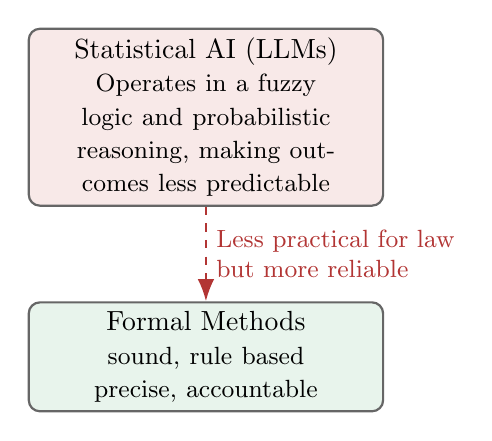
\begin{tikzpicture}[
    box/.style={rounded corners=4pt, draw=black!60, thick, minimum width=4.5cm, minimum height=1.1cm, align=center},
    arr/.style={-{Latex[length=2.8mm]}, thick, black!65}
  ]
  \node[box, fill=SoftRed, text width=4.2cm] (ai) {Statistical AI (LLMs)\\ \small Operates in a fuzzy logic and probabilistic reasoning, making outcomes less predictable};
  \node[box, fill=SoftGreen, text width=4.2cm, below=12mm of ai] (fm) {Formal Methods\\ \small sound, rule based precise, accountable};
  \draw[arr, dashed, ConflictRed] (ai) -- node[right, align=left, font=\small] {Less practical for law \\ but more reliable} (fm);
  \end{tikzpicture}
}
\end{column}
\end{columns}
\end{frame}

% =====================================
% SLIDE 2 — Thesis Vision & Research Gap
% =====================================
\begin{frame}{Thesis Vision: The two families of formal methods applied to Normative reasoning}

\centering
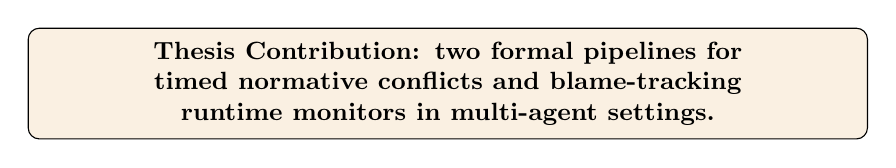
\begin{tikzpicture}
  \node[draw,rounded corners,fill=SoftOrange,text width=0.85\textwidth,align=center,inner sep=5pt,font=\small\bfseries] {
  Thesis Contribution: two formal pipelines for timed normative conflicts and blame-tracking runtime monitors in multi-agent settings.
  };
\end{tikzpicture}
\vspace{4mm}
\begin{columns}[T]
  \begin{column}{0.48\textwidth}
    \begin{block}{\textcolor{ConflictBlue}{Before Adoption \textemdash\ Static Analysis}}
      \small
      \emph{Normative specifications} combine obligations, prohibitions, and time constraints.\medskip

      \textbf{Problem:}  Conflicting norms may be \emph{hidden} inside complex temporal conditions, we suggest a novel characterization of timed normative conflicts through quantifiable conflict density measure,  quantifies their density, or resolves them automatically.
    \end{block}
  \end{column}
  \begin{column}{0.48\textwidth}
    \begin{block}{\textcolor{ConflictGreen}{During Enforcement \textemdash\ Runtime Monitoring}}
      \small
      \emph{Collaborative contracts} require both parties to act in order to \emph{collaborate and not interfere}.\medskip

      \textbf{Problem:}  Standard monitors only report the \emph{first} failure.
      Open-ended contracts need \emph{cumulative accountability} and per-agent blame attribution over infinite horizons.
    \end{block}
  \end{column}
\end{columns}
\end{frame}

% =====================================
% PART I SEPARATOR
% =====================================
{
\setbeamercolor{background canvas}{bg=ConflictBlue}
\begin{frame}[plain]
  \vfill
  \centering
  \textcolor{white}{\Huge\bfseries Part I}\\[6mm]
  \textcolor{white!85}{\Large Reasoning about Metric-Timed Normative Conflicts }\\[3mm]
  \textcolor{white!70}{\large Micro Metric-Timed Normative Logic $\TDDLfm$}
  \vfill
\end{frame}
}



\begin{frame}{Intuitive understanding of normative conflicts}
\onslide<1->{
  \begin{block}{The Fundamental Intuition}
    \small
    \emph{``Normative conflicts occur when complying with one norm can lead to noncompliance with another.''}
    \vspace{1mm}
    
    \raggedleft\footnotesize \color{gray} --- H. Kelsen, \textit{General Theory of Norms} (1991)
  \end{block}
}
\vspace{3mm}
\onslide<2->{
  \begin{block}{Deontic Conflicts in Dynamic Settings over time}
    \small
    \emph{``A deontic conflict occurs when a set of obligations is jointly unsatisfiable over time, meaning that no trace can be constructed that complies with every obligation in the set.''}
    \vspace{1mm}
    
    \raggedleft\footnotesize \color{gray} --- S. Colombo Tosatto et al., \textit{DEON} (2014)
  \end{block}
}
\vspace{3mm}
\onslide<3->{
  \begin{block}{Conflicts via Satisfiability}
    \small
    \emph{``A normative conflict occurs when triggering a normative rule, either always or in some feasible situation, inevitably leads to the violation of one or more rules, because the rule set imposes incompatible requirements.''}
    \vspace{1mm}
    
    \raggedleft\footnotesize \color{gray} --- N. Feng et al., \textit{ICSE} (2024)
  \end{block}
}
\end{frame}


% =====================================
% SLIDE 3 — Research Questions (Conflict)
% =====================================
\begin{frame}{Research Questions \textemdash\ Conflict Analysis}
\begin{enumerate}[\bfseries RQ1.]
  \item \textbf{Unsatisfiability and Conflict:}\quad Is every unsatisfiable formula necessarily a conflict?  Conversely, does a conflict imply unsatisfiability?

  \medskip
  \item \textbf{Conflict Quantification:}\quad Can we define a \emph{measure for the degree of conflict} within a specification?

  \medskip
  \item \textbf{Semantics-Preserving Resolution:}\quad Can we always resolve conflicts without altering the intended compliant behaviours. What are the properties of such resolutions?
\end{enumerate}


\end{frame}


% =====================================
% SLIDE 3 — Conflict Motivation
% ===================================
\begin{frame}{Motivation: Inpterpreting Timed norms as a Planning Problem}
\begin{columns}[T]
  \begin{column}{0.52\textwidth}
    \small
    \textbf{Use case:} Goods delivery to a harbour.

    \begin{itemize}
      \item \DC: Deliver between 09:00--16:00 to gate \textbf{or} parking.
      \item \SR: Parking \textbf{prohibited} 10:00--14:00.
      \item \MA: Gate \textbf{prohibited} 02:00--04:00, 08:00--24:00.
    \end{itemize}


    Conflicts are not logical contradictions in isolation: they arise from \emph{overlapping activation windows} and \emph{single-action capacity}.

    \medskip
    \textbf{Conflict at a specific time point t:}
    \begin{enumerate}
      \item \textcolor{ConflictRed}{\textbf{Deontic:}} Two contradictory obligations/prohibitions specified at the same t.
      \item \textcolor{ConflictOrange}{\textbf{Ontic:}} Two obliged actions cannot be performed at the same time t.
    \end{enumerate}
  \end{column}
  \begin{column}{0.45\textwidth}
    \centering
    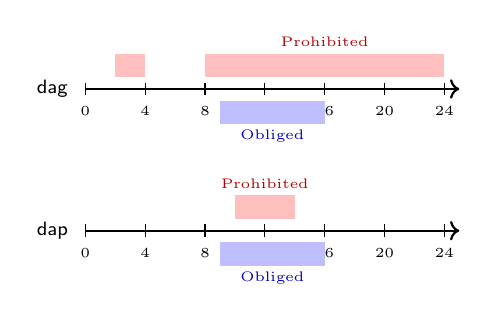
\begin{tikzpicture}[x=0.19cm,y=1cm,font=\tiny]
      % Gate timeline
      \draw[->,thick] (0,1.8) -- (25,1.8);
      \foreach \h in {0,4,8,12,16,20,24} {
        \draw (\h,1.72) -- (\h,1.88);
        \node[below] at (\h,1.7) {\h};
      }
      \node[left,font=\scriptsize] at (-0.5,1.8) {\delAtGate};

      % Gate F: [2,4],[8,24]
      \fill[red!25] (2,1.95) rectangle (4,2.25);
      \fill[red!25] (8,1.95) rectangle (24,2.25);
      \node[font=\tiny,red!70!black] at (16,2.4) {Prohibited};

      % Gate O: [9,16]
      \fill[blue!25] (9,1.35) rectangle (16,1.65);
      \node[font=\tiny,blue!70!black] at (12.5,1.2) {Obliged};

      % Overlap highlight [9,16]
      %\draw[ConflictRed,ultra thick,decorate,decoration={brace,amplitude=3pt,mirror}]
      %(9,2.5) -- (16,2.5) node[midway,above=3pt,font=\tiny\bfseries,ConflictRed] {Deontic conflict};

      % Park timeline
      \draw[->,thick] (0,0) -- (25,0);
      \foreach \h in {0,4,8,12,16,20,24} {
        \draw (\h,-0.08) -- (\h,0.08);
        \node[below] at (\h,-0.1) {\h};
      }
      \node[left,font=\scriptsize] at (-0.5,0) {\delAtPark};

      % Park F: [10,14]
      \fill[red!25] (10,0.15) rectangle (14,0.45);
      \node[font=\tiny,red!70!black] at (12,0.6) {Prohibited};

      % Park O: [9,16]
      \fill[blue!25] (9,-0.45) rectangle (16,-0.15);
      \node[font=\tiny,blue!70!black] at (12.5,-0.6) {Obliged};
    \end{tikzpicture}
  \end{column}
\end{columns}
\end{frame}



% =====================================
% SLIDE 5 — Methodology (Conflict)
% =====================================
\begin{frame}{Methodology: The $\TDDLfm$ Pipeline}
\begin{center}
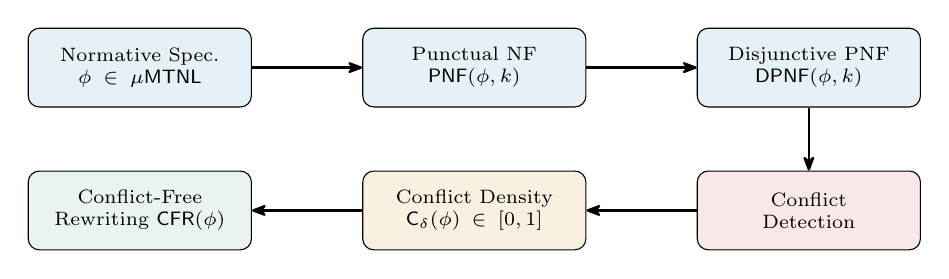
\begin{tikzpicture}[
  node distance=10mm and 14mm,
  box/.style={rectangle, draw, rounded corners, text width=26mm, align=center, minimum height=10mm, font=\scriptsize},
  arr/.style={-{Stealth[round]}, thick}
]
  \node[box, fill=SoftBlue] (spec) {Normative Spec.\\$\phi \in \TDDLfm$};
  \node[box, fill=SoftBlue, right=of spec] (pnf) {Punctual NF\\$\pnf(\phi,k)$};
  \node[box, fill=SoftBlue, right=of pnf] (dpnf) {Disjunctive PNF\\$\dpnf(\phi,k)$};
  \node[box, fill=SoftRed, below=8mm of dpnf] (detect) {Conflict\\Detection};
  \node[box, fill=SoftOrange, left=of detect] (density) {Conflict Density\\$\cd(\phi) \in [0,1]$};
  \node[box, fill=SoftGreen, left=of density] (cfr) {Conflict-Free\\Rewriting $\Namb(\phi)$};

  \draw[arr] (spec) -- (pnf);
  \draw[arr] (pnf) -- (dpnf);
  \draw[arr] (dpnf) -- (detect);
  \draw[arr] (detect) -- (density);
  \draw[arr] (density) -- (cfr);
\end{tikzpicture}
\end{center}

\smallskip
\begin{columns}[T]
\begin{column}{0.48\textwidth}
  \small
  \begin{itemize}
    \item Action-based trace semantics: each timed event carries \emph{exactly one action}.
    \item Time constraints encoded as \textbf{canonical interval sets} $\is$.
    \item Normalization decomposes intervals into \emph{punctual atoms}.
  \end{itemize}
\end{column}
\begin{column}{0.48\textwidth}
  \small
  \begin{itemize}
    \item Conflict detection via pattern matching on product terms of the \dpnf.
    \item Structural invariants literal ancestor preservation to ensure no spurious conflicts are introduced.
    \item Exponential worst-case blowup $\Rightarrow$ mitigated by  conflict calculus.
  \end{itemize}
\end{column}
\end{columns}
\end{frame}

% =====================================
% SLIDE 6 — Answering RQ1–RQ3
% =====================================
\begin{frame}{Answering the Research Questions}
\small
\begin{columns}[T]
  \begin{column}{0.32\textwidth}
  \begin{block}{Q2: Conflict Density}
    \[
    \cd(\phi) := \frac{|\text{CPT in } \dpnf(\phi)|}{|\text{PT in } \dpnf(\phi)|}
    \]
    \begin{itemize}\setlength\itemsep{2pt}
      \item $\cd = 0$: conflict-free.
      \item $\cd = 1$: fully conflicting.
      \item Use case: $\cd(\UC) \approx 0.81$.
    \end{itemize}
  \end{block}
\end{column}
\begin{column}{0.32\textwidth}
  \begin{block}{RQ1: Exact Characterisation}
    \centering
    \vspace{2mm}
    $\phi$ is unsat $\;\Longleftrightarrow\;$ $\cd(\phi) = 1$
    \vspace{2mm}

    \raggedright
    \textbf{Key results:}
    \begin{itemize}\setlength\itemsep{2pt}
      \item Punctual conflicts $=$ MUS over punctual literals.
      \item Only deontic \& ontic patterns exist.
    \end{itemize}
  \end{block}
\end{column}

\begin{column}{0.32\textwidth}
  \begin{block}{RQ3: Conflict-Free Rewriting}
    If $\cd(\phi) < 1$:
    
      $\quad \exists\;\phi' \equiv \phi,\quad \cd(\phi') = 0$
    
    \begin{itemize}\setlength\itemsep{2pt}
      \item Prune conflicting terms.
      \item Compactness cost: up to $\mathcal{O}(2^{|\phi|})$.
      \item Conflict calculus for manual big-step reasoning.
    \end{itemize}
  \end{block}
\end{column}
\end{columns}
\end{frame}

% =====================================
% SLIDE 7 — The Overall Framework (Conflict)
% =====================================
\begin{frame}{The Conflict Analysis \& Resolution Framework}
\begin{center}
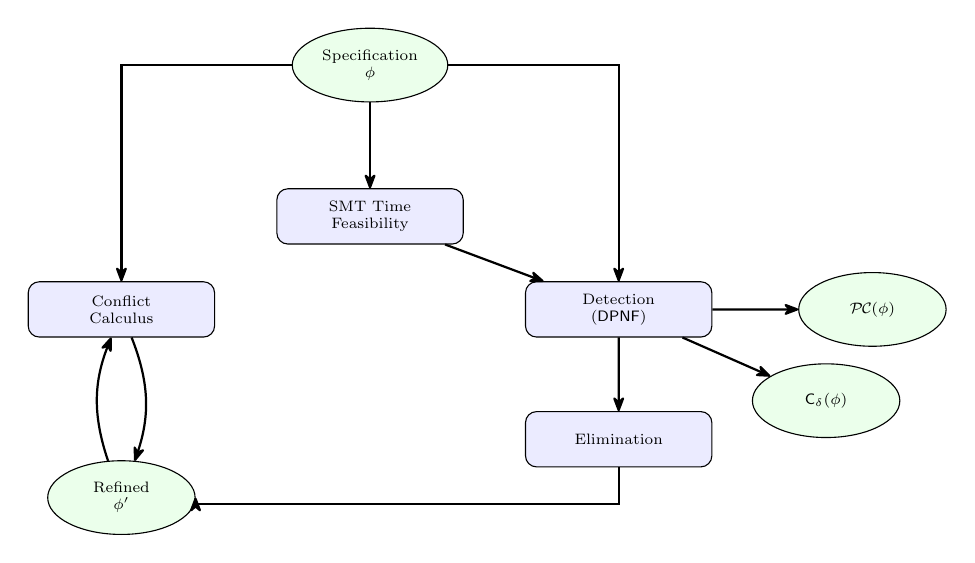
\begin{tikzpicture}[
  node distance=14mm and 16mm,
  rect/.style={rectangle, draw, rounded corners, text width=28mm, align=center, minimum height=9mm, fill=blue!8, font=\scriptsize},
  ell/.style={ellipse, draw, minimum width=24mm, minimum height=12mm, align=center, fill=green!8, font=\scriptsize},
  arr/.style={-{Stealth[round]}, thick},
  scale=0.78, transform shape
]
  \node[ell] (spec) {Specification\\$\phi$};
  \node[rect, below=of spec] (smt) {SMT Time\\Feasibility};
  \node[rect, below left=6mm and 10mm of smt] (calc) {Conflict\\Calculus};
  \node[rect, below right=6mm and 10mm of smt] (det) {Detection\\(\dpnf)};
  \node[rect, below=12mm of det] (elim) {Elimination};
  \node[ell, right=14mm of det] (pc) {$\mathcall{PC}(\phi)$};
  \node[ell, below right=6mm and 10mm of det] (cdens) {$\cd(\phi)$};
  \node[ell, below=20mm of calc] (ref) {Refined\\$\phi'$};

  \draw[arr] (spec) -- (smt);
  \draw[arr] (spec.west) -| (calc.north);
  \draw[arr] (spec.east) -| (det.north);
  \draw[arr] (smt) -- (det);
  \draw[arr] (det) -- (pc);
  \draw[arr] (det) -- (elim);
  \draw[arr] (det) -- (cdens);
  \draw[arr] (elim.south) -- ++(0,-0.6) -| (ref.east);
  \draw[arr] (calc) to[bend left=20] (ref);
  \draw[arr] (ref) to[bend left=20] (calc);
\end{tikzpicture}
\end{center}
\end{frame}

% =====================================
% PART II SEPARATOR
% =====================================
{
\setbeamercolor{background canvas}{bg=ConflictGreen}
\begin{frame}[plain]
  \vfill
  \centering
  \textcolor{white}{\Huge\bfseries Part II}\\[6mm]
  \textcolor{white!85}{\Large  Reasoning about Blame in Multi-Party Collaborative Contracts }\\[3mm]
  \textcolor{white!70}{\large Two-Agent Collaborative Normative Logic \cDL}
  \vfill
\end{frame}
}

% =====================================
% SLIDE 8 — Contract Motivation
% =====================================
\begin{frame}{Motivation: Collaborative Contracts \& the Accountability Gap}
\begin{columns}[T]
\begin{column}{0.55\textwidth}
  \small
  \textbf{Example:  Flat rental agreement.}
  \begin{itemize}
    \item \emph{Payment} needs tenant's offer \textbf{and} landlord's acceptance.
    \item \emph{Occupancy} requires landlord to grant access.
    \item Violations may be \emph{repaired} (pay a fine).
    \item Contract repeats \emph{every month}, unless terminated with a 3 months notice.
  \end{itemize}

  \medskip
  \textbf{Key challenges:}
  \begin{enumerate}
    \item Distinguish \textbf{attempts} from \textbf{outcomes}.
    \item Attribute \textbf{blame} (who blocked whom?).
    \item Monitor \textbf{open-ended} contracts.
    \item Provide \textbf{cumulative} accountability, not just first-failure.
  \end{enumerate}
\end{column}
\begin{column}{0.42\textwidth}
  \centering
  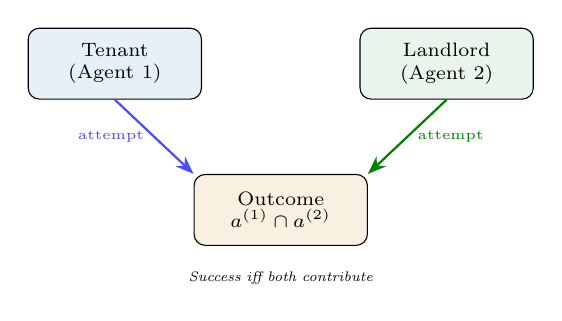
\begin{tikzpicture}[
    node distance=8mm,
    agbox/.style={draw, rounded corners, minimum width=22mm, minimum height=9mm, font=\scriptsize, align=center},
    arr/.style={-{Stealth}, thick}
  ]
    \node[agbox, fill=SoftBlue] (t) {Tenant\\(Agent 1)};
    \node[agbox, fill=SoftGreen, right=20mm of t] (l) {Landlord\\(Agent 2)};
    \node[agbox, fill=SoftOrange, below=14mm of $(t)!0.5!(l)$] (out) {Outcome\\$a^{(1)} \cap a^{(2)}$};

    \draw[arr,blue!70] (t.south) -- (out.north west) node[midway,left,font=\tiny] {attempt};
    \draw[arr,green!50!black] (l.south) -- (out.north east) node[midway,right,font=\tiny] {attempt};
    \node[below=2mm of out,font=\tiny\itshape,text width=35mm,align=center] {Success iff both contribute};
  \end{tikzpicture}

  \vspace{4mm}
  \small
  \textbf{Formalisation:}
  $\Sigma = \Sigma_C^{(1)} \cup \Sigma_C^{(2)}$\\
  letters $A \in 2^{\Sigma}$, traces $\pi \in (2^\Sigma)^*$.
\end{column}
\end{columns}
\end{frame}

% =====================================
% SLIDE 9 — Research Questions (Contract)
% =====================================
% \begin{frame}{Research Questions \textemdash\ Collaborative Contract Monitoring}
% \begin{enumerate}[\bfseries RQ1.]
%   \item How can \textbf{collaboration} be modeled as a first-class semantic object, distinguishing individual \emph{attempts} from jointly successful \emph{outcomes}?

%   % \medskip
%   % \item Which \textbf{trace abstractions} effectively capture cooperative behaviour and \emph{non-interference} at the granularity of contractual periods?

%   % \medskip
%   % \item How can open-ended, potentially \textbf{infinite}, streams of duties and rights be \emph{specified and monitored}?

%   \medskip
%   \item How can \textbf{blame and quantitative accountability} be defined to support automated monitoring beyond first-failure?
% \end{enumerate}
% \end{frame}

% =====================================
% SLIDE 10 — Methodology (Contract)
% =====================================
\begin{frame}{Methodology: A Four-Phase Pipeline}
\begin{center}
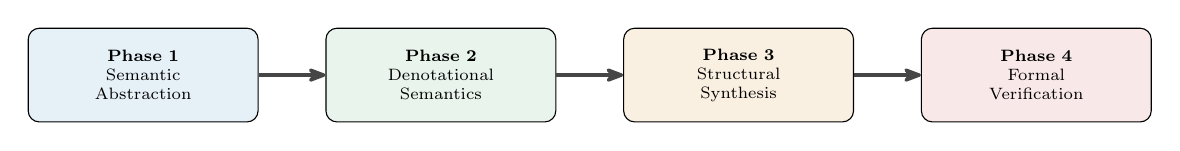
\begin{tikzpicture}[
  phase/.style={draw, rounded corners, text width=32mm, align=center, minimum height=14mm, font=\scriptsize},
  arr/.style={-{Stealth[round]}, very thick, ConflictGray},
  node distance=6mm and 10mm, scale=0.85, transform shape
]
  \node[phase, fill=SoftBlue] (p1) {\textbf{Phase 1}\\Semantic\\Abstraction};
  \node[phase, fill=SoftGreen, right=of p1] (p2) {\textbf{Phase 2}\\Denotational\\Semantics};
  \node[phase, fill=SoftOrange, right=of p2] (p3) {\textbf{Phase 3}\\Structural\\Synthesis};
  \node[phase, fill=SoftRed, right=of p3] (p4) {\textbf{Phase 4}\\Formal\\Verification};

  \draw[arr] (p1) -- (p2);
  \draw[arr] (p2) -- (p3);
  \draw[arr] (p3) -- (p4);
\end{tikzpicture}
\end{center}

\vspace{2mm}
\begin{columns}[T]
\begin{column}{0.48\textwidth}
  \small
  \begin{itemize}
    \item \textbf{P1:} Multi-layered trace model with attempt-based interaction ($\Sigma_C^{(i)}$).
    \item \textbf{P2:} Semantics-first for blame and satisfaction: forward looking and quantitative. (4 in total)
  \end{itemize}
\end{column}
\begin{column}{0.48\textwidth}
  \small
  \begin{itemize}
    \item \textbf{P3:} Compile \cDL contracts into deterministic Moore/Mealy machines by structural construction.
    \item \textbf{P4:} Conformance proofs: monitor output $\equiv$ denotational semantics for \emph{every} finite prefix.
  \end{itemize}
\end{column}
\end{columns}
\end{frame}

% =====================================
% SLIDE 11 — The cDL Logic
% =====================================
\begin{frame}{The Logic \cDL \textemdash\ Syntax}
\small
\begin{columns}[T]
\begin{column}{0.48\textwidth}
  \textbf{Literals (party $p \in \{1,2\}$, action $a$):}
  \[
  \ell ::= \obl[p]{a} \mid \frb[p]{a} \mid \perm[p]{a} \mid \top \mid \bot
  \]

  \textbf{Contract operators:}
  \[
  C ::= \ell \mid C \wedge C' \mid C\,;\,C' \mid C \repair C'
  \]

  \textbf{Repetition:}
  \[
  C^n \quad\text{(finite)}\qquad \repit{C} \quad\text{(unbounded)}
  \]
\end{column}
\begin{column}{0.48\textwidth}
  \textbf{Regular expression control:}
  \[
  \trig[re]{C} \quad\text{(trigger)} \qquad \guard[re]{C} \quad\text{(guard)}
  \]

  \medskip
  \textbf{Running example:}
  \begin{align*}
    C_2 &:= \perm[\text{Ten}]{\OCC}  &\text{(right to occupy)}\\
    C_3 &:= \obl[\text{Ten}]{\PAY} \repair \obl[\text{Ten}]{\PAYF} &\text{(pay or fine)}\\
    C   &:= \guard[\Gamma^+ \!\cdot\! \notifterm^{(1)}]{\repit{C_2 \wedge C_3}}
  \end{align*}
\end{column}
\end{columns}
\end{frame}



% =====================================
% SLIDE 12 — Five-Valued Forward-Looking Semantics
% =====================================
\begin{frame}{Five-Valued Forward-Looking Satisfiaction Semantics \textemdash\ $\tightverdicts$}
\small
\begin{columns}[T]
\begin{column}{0.55\textwidth}
  \textbf{Core idea:} Identify the \emph{unique decisive prefix} where a contract becomes irrevocably satisfied or violated.

  \[
  \tightverdicts = \{\;\underbrace{?}_{\text{pending}},\;\;
    \underbrace{\topt}_{\text{tight sat}},\;\;
    \underbrace{\bott}_{\text{tight viol}},\;\;
    \underbrace{\topp}_{\text{post-sat}},\;\;
    \underbrace{\botp}_{\text{post-viol}}\;\}
  \]

  \begin{itemize}
    \item $\pi \satt C$: \emph{first} prefix where $C$ is satisfied (acceptance frontier).
    \item $\pi \violt C$: \emph{first} prefix where $C$ is violated (rejection frontier).
    \item $\pi \presat C$: no frontier reached yet.
    \item $\pi \postsat C$ / $\pi \postviol C$: past the decisive point.
  \end{itemize}
\end{column}
\begin{column}{0.42\textwidth}
  \centering
  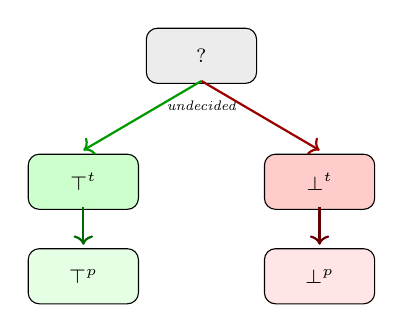
\begin{tikzpicture}[
    x=10mm, y=8mm,
    reg/.style={draw, rounded corners, minimum width=14mm, minimum height=7mm, font=\scriptsize, align=center}
  ]
    \node[reg, fill=gray!15] at (0,3) {$?$};
    \node at (0,2.2) {\tiny\itshape undecided};

    \node[reg, fill=green!20] at (-1.5,1) {$\topt$};
    \node[reg, fill=red!20]   at (1.5,1)  {$\bott$};

    \node[reg, fill=green!10] at (-1.5,-0.5) {$\topp$};
    \node[reg, fill=red!10]   at (1.5,-0.5)  {$\botp$};

    \draw[->,thick,green!60!black] (0,2.6) -- (-1.5,1.5);
    \draw[->,thick,red!60!black]   (0,2.6) -- (1.5,1.5);
    \draw[->,thick,green!40!black] (-1.5,0.6) -- (-1.5,0);
    \draw[->,thick,red!40!black]   (1.5,0.6) -- (1.5,0);
  \end{tikzpicture}

  \vspace{2mm}
  \textbf{Theorem:} The five regions are \emph{pairwise disjoint} and \emph{jointly exhaustive}.
\end{column}
\end{columns}
\end{frame}

% =====================================
% SLIDE 13 — Five-Valued Semantics: Operators
% =====================================
\begin{frame}{Tight Semantics for Contract Operators}
\small
\begin{columns}[T]
\begin{column}{0.48\textwidth}
  \textbf{Literals} (decided in one step):
  \begin{align*}
    \trace{A} \satt \obl[1]{a} &\mydef \{a^{(1)},a^{(2)}\} \subseteq A\\
    \trace{A} \violt \obl[1]{a} &\mydef \{a^{(1)},a^{(2)}\} \not\subseteq A
  \end{align*}

  \textbf{Conjunction} $C \wedge C'$:
  \begin{itemize}
    \item Satisfaction: both succeed; decisive index = $\max(k,k')$.
  \end{itemize}

  \textbf{Sequence} $C\,;\,C'$:
  \begin{itemize}
    \item Split witness $k$: $C$ on $[1,k]$, then $C'$ on $[k{+}1,s]$.
  \end{itemize}
\end{column}
\begin{column}{0.48\textwidth}
  \textbf{Reparation} $C \repair C'$:
  \begin{align*}
    \pi \satt C \repair C' &\mydef \pi \satt C \;\sor\\
      &\quad \exists k: \pi_k \violt C \nd \pi^k \satt C'
  \end{align*}

  \textbf{Repetition} $\repit{C}$:
  \begin{itemize}
    \item $\repit{C}$ is \emph{never} tightly satisfied on finite traces.
  \end{itemize}

  \textbf{Guard/Trigger:}
  \begin{itemize}
    \item $\guard[re]{C}$: $C$ enforced while $re$ is possible.
    \item $\trig[re]{C}$: $C$ activated once $re$ matches.
  \end{itemize}
\end{column}
\end{columns}

\vspace{2mm}
\centering
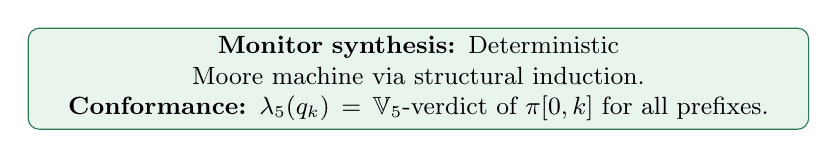
\begin{tikzpicture}
  \node[draw=ConflictGreen,rounded corners,fill=SoftGreen,text width=0.8\textwidth,align=center,inner sep=3pt,font=\small] {
  \textbf{Monitor synthesis:} Deterministic Moore machine via structural induction.\\
  \textbf{Conformance:} $\lambda_5(q_k) = \tightverdicts$-verdict of $\pi[0,k]$ for all prefixes.
  };
\end{tikzpicture}
\end{frame}

% =====================================
% SLIDE 14 — Eleven-Valued Blame Semantics
% =====================================
\begin{frame}{Eleven-Valued Forward-Looking Blame Semantics \textemdash\ $\mathbb{V}_{11}$}
\small
\begin{columns}[T]
\begin{column}{0.55\textwidth}
  \textbf{Refinement:} Split each violation verdict by \emph{who} is responsible.

  \[
  \mathbb{V}_{11} =
    \underbrace{\{?,\;\topt,\;\topp\}}_{\text{unchanged}}
    \;\cup\;
    \underbrace{\{\bot^t_S,\;\bot^p_S \mid S \subseteq \{1,2\}\}}_{\text{blame-indexed}}
  \]

  \textbf{Blame rules for literals:}
  \begin{align*}
    \trace{A} \vDash_{\bottp{p}} \obl[p]{a}
      &\mydef a^{(p)} \notin A\\[-2pt]
      &\quad\text{(subject did not attempt)}\\[4pt]
    \trace{A} \vDash_{\bottp{\bar{p}}} \obl[p]{a}
      &\mydef a^{(p)} \in A \wedge a^{(\bar{p})} \notin A\\[-2pt]
      &\quad\text{(counterparty withheld)}
  \end{align*}
\end{column}
\begin{column}{0.42\textwidth}
  \textbf{Conjunction blame propagation:}
  \begin{itemize}
    \item Both $C_1, C_2$ violate $\Rightarrow$ $S = S_1 \cup S_2$.
  \end{itemize}

  \medskip
  \textbf{Key properties:}
  \begin{enumerate}
    \item Joint blame $\{1,2\}$ arises only via conjunction.
    \item Blame monitor $\mathcal{M}_{11}$: same states \& transitions as $\mathcal{M}_5$, only $\lambda_5 \to \lambda_{11}$.
  \end{enumerate}

  \vspace{2mm}
  \textbf{Theorem:} $\lambda_{11}$ is a \emph{consistency-preserving refinement} of $\lambda_5$.
\end{column}
\end{columns}
\end{frame}

% =====================================
% SLIDE 15 — Limitation of Forward Blame
% =====================================
\begin{frame}{Limitation: The First-Failure Ceiling}
\begin{columns}[T]
\begin{column}{0.55\textwidth}
  \small
  The forward-looking blame monitor detects the \textbf{first decisive violation} and then enters a \emph{permanent sink} $\botpp{S}$.

  \medskip
  \textbf{Consequence for $\repit{C_3}$:}
  \begin{itemize}
    \item If tenant is blamed for missing a fine $\Rightarrow$ monitor stays in $\botpp{1}$ forever.
    \item Even if landlord subsequently blocks a payment, the verdict is \emph{frozen}.
  \end{itemize}

  \medskip
  
\begin{tikzpicture}
    \node[draw=ConflictRed,rounded corners,fill=SoftRed,text width=0.92\linewidth,align=center,inner sep=4pt,font=\small] {
    \textbf{Problem:}\; Open-ended contracts need \emph{cumulative} blame over the full interaction lifespan.
    };
  \end{tikzpicture}

  \vspace{3mm}
  $\Longrightarrow$ \textbf{Solution:} Quantitative semantics with scalar and vector domains.
\end{column}
\begin{column}{0.42\textwidth}
  \centering
  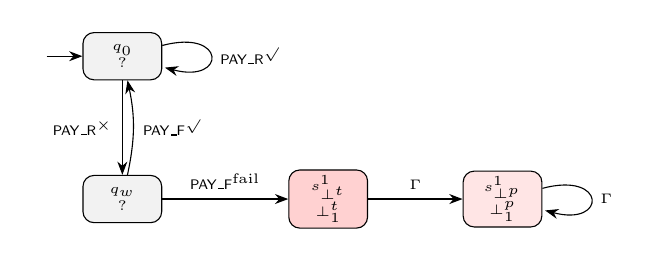
\begin{tikzpicture}[
    ->, >=Stealth, node distance=12mm,
    every state/.style={rectangle, rounded corners, draw, minimum width=10mm, minimum height=6mm, inner sep=2pt, font=\tiny, align=center},
    initial text={}
  ]
    \node[initial,state,fill=gray!10] (q0) {$q_0$\\$?$};
    \node[state,fill=gray!10,below=of q0] (qw) {$q_w$\\$?$};
    \node[state,fill=red!18,right=16mm of qw] (qv) {$s_{\bott}^1$\\$\bottp{1}$};
    \node[state,fill=red!10,right=12mm of qv] (qpv) {$s_{\botp}^1$\\$\botpp{1}$};

    \path (q0) edge[loop right] node[right,font=\tiny] {$\PAY^\surd$} ()
          (q0) edge node[left,font=\tiny] {$\PAY^\times$} (qw)
          (qw) edge[bend right=12] node[right,font=\tiny] {$\PAYF^\surd$} (q0)
          (qw) edge node[above,font=\tiny] {$\PAYF^{\text{fail}}$} (qv)
          (qv) edge node[above,font=\tiny] {$\Gamma$} (qpv)
          (qpv) edge[loop right] node[font=\tiny] {$\Gamma$} ();
  \end{tikzpicture}

  \vspace{2mm}
  \scriptsize Blame monitor for $\repit{C_3}$: once $\botpp{1}$ is reached, it \emph{never} leaves.
\end{column}
\end{columns}
\end{frame}

% =====================================
% SLIDE 16 — Contract Progress Monitor
% =====================================
\begin{frame}{Contract Progress Monitor \textemdash\ $\Prog$}
\small
\textbf{Key idea:} A \emph{derivative operator} that computes the \textbf{reachable residual contract} after each event.

\[
\Prog : \Gamma^* \times \cDL \to \cDL \cup \{\emptc\}
\]

\begin{columns}[T]
\begin{column}{0.48\textwidth}
  \textbf{Selected clauses:}
  \begin{align*}
    \Prog(\trace{A},\;\ell) &:= \emptc \quad\text{(literal consumed)}\\
    \Prog(\trace{A},\;C_1 \wedge C_2) &:= \Prog(\trace{A},C_1) \wedge \Prog(\trace{A},C_2)\\
    \Prog(\trace{A},\;\repit{C}) &:= \Prog(\trace{A},C)\;;\;\repit{C}
  \end{align*}

  \textbf{Reparation (semantic branching):}
  \[
  \Prog(\trace{A},\;C_1 \repair C_2) :=
    \begin{cases}
      \Prog(\trace{A},C_1) \repair C_2 & \text{if } \trace{A} \presat C_1\\
      \Prog(\trace{A},C_2) & \text{if } \trace{A} \violt C_1\\
      \emptc & \text{if } \trace{A} \satt C_1
    \end{cases}
  \]
\end{column}
\begin{column}{0.48\textwidth}
  \textbf{Trace example on $\repit{C_3}$:}
  \begin{center}
  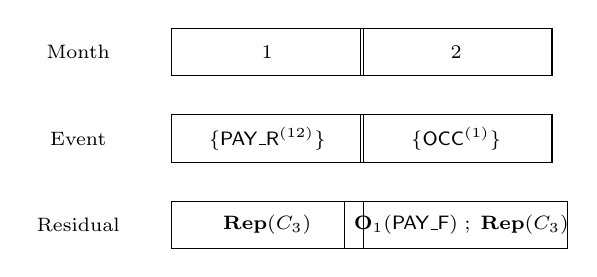
\begin{tikzpicture}[y=1.1cm, x=2.4cm, font=\scriptsize]
    \tikzset{cell/.style={draw, rectangle, text width=22mm, minimum height=6mm, align=center}}

    \node at (0,0) {Month};
    \node at (0,-1) {Event};
    \node at (0,-2) {Residual};

    \node[cell] at (1,0) {$1$};
    \node[cell] at (2,0) {$2$};

    \node[cell] at (1,-1) {$\{\PAY^{(12)}\}$};
    \node[cell] at (2,-1) {$\{\OCC^{(1)}\}$};

    \node[cell] at (1,-2) {$\repit{C_3}$};
    \node[cell,text width=26mm] at (2,-2) {$\obl[1]{\PAYF}\;;\;\repit{C_3}$};
  \end{tikzpicture}
  \end{center}

  \vspace{2mm}
  \textbf{Finiteness:} $\rrcs{C}$ is finite $\Rightarrow$ Mealy machine is \emph{finite-state}.
\end{column}
\end{columns}
\end{frame}

% =====================================
% SLIDE 17 — Quantitative Violation (Singleton)
% =====================================
\begin{frame}{Quantitative Violation Semantics \textemdash\ Singleton Domain $\mathbb{N}$}
\small
\begin{columns}[T]
\begin{column}{0.55\textwidth}
  \textbf{Transition:} From ``Did it fail?'' to ``How many times did it fail?''

  \[
  \qsem{\cdot} : \Gamma^* \times \cDL \to \mathbb{N}
  \]

  \textbf{Recursive accumulation:}
  \[
  \qsem{\trace{A} \circ \pi,\; C} :=
    \underbrace{\qsem{\trace{A},\;C}}_{\text{instant penalty}}
    +
    \underbrace{\qsem{\pi,\;\Prog(\trace{A},C)}}_{\text{suffix score}}
  \]

  \textbf{Instantaneous score:}
  \[
  \qsem{\trace{A},\;C} :=
  \begin{cases}
    \qsem{\trace{A},C_1} + \qsem{\trace{A},C_2} & C = C_1 \wedge C_2\\
    1 & \trace{A} \violt \LH(C)\\
    0 & \text{otherwise}
  \end{cases}
  \]
\end{column}
\begin{column}{0.42\textwidth}
  \textbf{Key properties:}
  \begin{itemize}
    \item $\qsem{\pi,C} = 0$ $\Leftrightarrow$ $\pi$ is fully compliant ($\presat$, $\satt$, or $\postsat$).
    \item $\qsem{\pi,C} > 0$ even when $\pi \satt C$ (through reparation) $\Rightarrow$ \emph{cost of repair visible}.
    \item Monotonically increasing along prefixes.
  \end{itemize}

  \vspace{3mm}
  \textbf{Monitor:} Mono-Quantitative Mealy machine $\qmc(C)$.
  \[
  \lambda(q,A) := \qsem{\trace{A},\;q}
  \]
  \textbf{Theorem:} $\qscore(\qmc(C),\pi) = \qsem{\pi,C}$.
\end{column}
\end{columns}
\end{frame}

% =====================================
% SLIDE 18 — Quantitative Blame (Vector)
% =====================================
\begin{frame}{Quantitative Blame Semantics \textemdash\ Vector Domain $\mathbb{N}^2$}
\small
\begin{columns}[T]
\begin{column}{0.55\textwidth}
  \textbf{Refinement:} Replace scalar $\mathbb{N}$ by agent-indexed vectors.
  \[
  \qblame{\cdot} : \Gamma^* \times \cDL \to \mathbb{N}^2
  \]

  \textbf{Instantaneous blame:}
  \[
  \qblame{\trace{A},\;C} :=
  \begin{cases}
    \qblame{\trace{A},C_1} + \qblame{\trace{A},C_2} & C = C_1 \wedge C_2\\[4pt]
    (1,0) & \trace{A} \vDash_{\bottp{1}} \LH(C)\\
    (0,1) & \trace{A} \vDash_{\bottp{2}} \LH(C)\\
    (0,0) & \text{otherwise}
  \end{cases}
  \]

  \textbf{No $(1,1)$ at literal level:} blame verdicts are mutually exclusive per literal.
  Joint blame $(1,1)$ arises only through \emph{conjunction} over distinct literals.
\end{column}
\begin{column}{0.42\textwidth}
  \textbf{Example:} $\perm[1]{\OCC} \wedge \obl[1]{\PAY}$,
  $A = \{\OCC^{(1)}\}$:
  \begin{align*}
    \qblame{\trace{A},\;\perm[1]{\OCC}} &= (0,1)\\
    \qblame{\trace{A},\;\obl[1]{\PAY}} &= (1,0)\\
    \qblame{\trace{A},\;C_2 \wedge C_3} &= (1,1)
  \end{align*}

  \vspace{2mm}
  \textbf{Decomposition lemma:}
  \[
  \qsem{\pi,C} = n_1 + n_2
  \quad\text{where}\quad
  \qblame{\pi,C} = (n_1,n_2)
  \]
  $\Rightarrow$ Blame is a \emph{finer view} of the same violation count.
\end{column}
\end{columns}
\end{frame}

% =====================================
% SLIDE 19 — Double-Quantitative Monitor
% =====================================
\begin{frame}{Double-Quantitative Monitor \textemdash\ $\qbm(C)$}
\small
\begin{columns}[T]
\begin{column}{0.52\textwidth}
  \textbf{Definition:} Mealy machine with output in $\mathbb{N}^2$.
  \[
  \qbm(C) := (Q,\;q_0,\;\Gamma,\;\delta,\;\lambda_{\mathbb{N}^2})
  \]
  \begin{itemize}
    \item $Q := \rrcs{C}$, \quad $q_0 := C$
    \item $\delta(q,A) := \Prog(\trace{A},q)$
    \item $\lambda_{\mathbb{N}^2}(q,A) := \qblame{\trace{A},q}$
  \end{itemize}

  \textbf{Blame execution score:}
  \[
  \qscore(\qbm(C),\pi) = \sum_{i=0}^{|\pi|-1} \lambda_{\mathbb{N}^2}(q_i,A_i)
  \]

  \textbf{Conformance theorem:}
  \[
  \qscore(\qbm(C),\pi) = \qblame{\pi,C}
  \]
\end{column}
\begin{column}{0.45\textwidth}
  \centering
  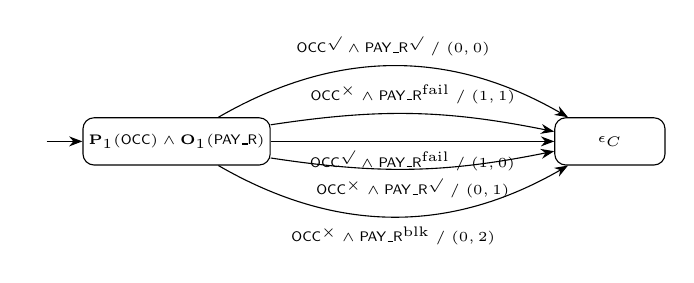
\begin{tikzpicture}[
    ->, >=Stealth, node distance=36mm,
    every state/.style={rectangle, rounded corners, draw, minimum width=14mm, minimum height=6mm, inner sep=2pt, font=\tiny, align=center},
    initial text={}
  ]
    \node[initial, state] (q0) {$\perm[1]{\OCC} \wedge \obl[1]{\PAY}$};
    \node[state, right=of q0] (qe) {$\emptc$};

    \path
      (q0) edge[bend left=30] node[above,font=\tiny] {$\OCC^\surd \wedge \PAY^\surd\;/\;(0,0)$} (qe)
      (q0) edge[bend left=10] node[above,font=\tiny] {$\OCC^\times \wedge \PAY^{\text{fail}}\;/\;(1,1)$} (qe)
      (q0) edge node[below,font=\tiny] {$\OCC^\surd \wedge \PAY^{\text{fail}}\;/\;(1,0)$} (qe)
      (q0) edge[bend right=10] node[below,font=\tiny] {$\OCC^\times \wedge \PAY^\surd\;/\;(0,1)$} (qe)
      (q0) edge[bend right=30] node[below,font=\tiny] {$\OCC^\times \wedge \PAY^{\text{blk}}\;/\;(0,2)$} (qe);
  \end{tikzpicture}

  \vspace{2mm}
  \scriptsize Fragment of $\qbm(\perm[1]{\OCC} \wedge \obl[1]{\PAY})$.\\
  Note: $(0,2)$ when \emph{both} violations blamed on agent~2.
\end{column}
\end{columns}
\end{frame}

% =====================================
% SLIDE 20 — The Full Semantic Hierarchy
% =====================================
\begin{frame}{The Full Semantic Hierarchy}
\begin{center}
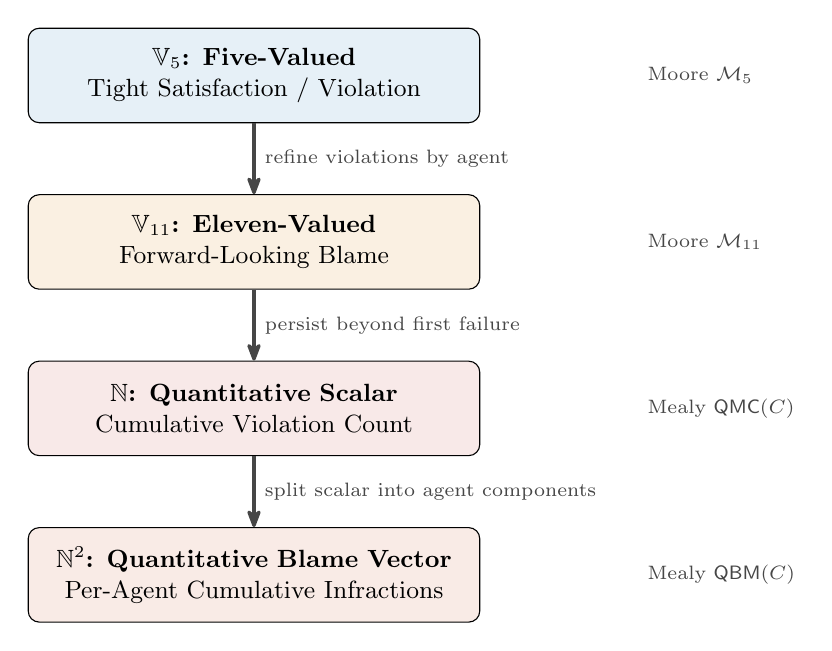
\begin{tikzpicture}[
  layer/.style={draw, rounded corners, text width=55mm, align=center, minimum height=12mm, font=\small},
  arr/.style={-{Stealth[round]}, very thick, ConflictGray},
  node distance=9mm
]
  \node[layer, fill=SoftBlue]   (v5) {\textbf{$\mathbb{V}_5$: Five-Valued}\\Tight Satisfaction / Violation};
  \node[layer, fill=SoftOrange, below=of v5] (v11) {\textbf{$\mathbb{V}_{11}$: Eleven-Valued}\\Forward-Looking Blame};
  \node[layer, fill=SoftRed, below=of v11] (qn) {\textbf{$\mathbb{N}$: Quantitative Scalar}\\Cumulative Violation Count};
  \node[layer, fill=SoftRed!70!SoftOrange, below=of qn] (qn2) {\textbf{$\mathbb{N}^2$: Quantitative Blame Vector}\\Per-Agent Cumulative Infractions};

  \draw[arr] (v5) -- node[right,font=\scriptsize] {refine violations by agent} (v11);
  \draw[arr] (v11) -- node[right,font=\scriptsize] {persist beyond first failure} (qn);
  \draw[arr] (qn) -- node[right,font=\scriptsize] {split scalar into agent components} (qn2);

  % Monitor labels
  \node[right=20mm of v5, font=\scriptsize, text=ConflictGray] {Moore $\mathcal{M}_5$};
  \node[right=20mm of v11, font=\scriptsize, text=ConflictGray] {Moore $\mathcal{M}_{11}$};
  \node[right=20mm of qn, font=\scriptsize, text=ConflictGray] {Mealy $\qmc(C)$};
  \node[right=20mm of qn2, font=\scriptsize, text=ConflictGray] {Mealy $\qbm(C)$};
\end{tikzpicture}
\end{center}

\vspace{2mm}
\centering
\small
\textbf{Each layer} has a \emph{denotational semantics} and a \emph{proven-correct monitor construction}.\\
$\qsem{\pi,C} = n_1 + n_2$ where $\qblame{\pi,C} = (n_1,n_2)$ \textemdash\ blame is a strict refinement of the violation count.
\end{frame}

% =====================================
% SLIDE 21 — Contributions Summary
% =====================================
\begin{frame}{Summary of Contributions}
\small
\begin{columns}[T]
\begin{column}{0.48\textwidth}
  \begin{block}{\textcolor{ConflictBlue}{Conflict Analysis ($\TDDLfm$)}}
    \begin{enumerate}
      \item Formal machinery: interval-set logic, \dpnf, conflict calculus.
      \item Exact characterisation: $\text{unsat} \Leftrightarrow \cd(\phi) = 1$.
      \item Conflict density metric $\cd(\phi) \in [0,1]$.
      \item Sound \& complete conflict-free rewriting $\Namb(\phi)$.
      \item Complexity bounds \& conciseness analysis.
    \end{enumerate}
  \end{block}
\end{column}
\begin{column}{0.48\textwidth}
  \begin{block}{\textcolor{ConflictGreen}{Contract Monitoring (\cDL)}}
    \begin{enumerate}
      \item Attempt-based interaction model.
      \item \cDL logic with repetition, guards, triggers, reparation.
      \item 5-valued tight satisfaction semantics + Moore monitors.
      \item 11-valued forward blame semantics + blame monitors.
      \item Quantitative scalar ($\mathbb{N}$) and vector ($\mathbb{N}^2$) blame monitors.
      \item Full pipeline: denotational $\to$ operational, with conformance proofs.
    \end{enumerate}
  \end{block}
\end{column}
\end{columns}
\end{frame}

% =====================================
% SLIDE 22 — Outlook
% =====================================
\begin{frame}{Outlook \& Future Work}
\begin{columns}[T]
\begin{column}{0.48\textwidth}
  \textbf{Extending $\TDDLfm$:}
  \begin{itemize}
    \item Actions with \emph{duration}.
    \item Conditional \& permission literals.
    \item Defeasibility mechanisms.
    \item Interaction frames (prevention / enabling / interference between actions).
  \end{itemize}
\end{column}
\begin{column}{0.48\textwidth}
  \textbf{Extending \cDL:}
  \begin{itemize}
    \item Constructive proof of $\rrcs{C}$ finiteness.
    \item $n$-agent generalisation ($\mathbb{N}^n$ blame vectors).
    \item Integration of static conflict analysis and dynamic monitoring.
    \item Tool development: solver + runtime monitor.
  \end{itemize}
\end{column}
\end{columns}

\vspace{5mm}
\centering
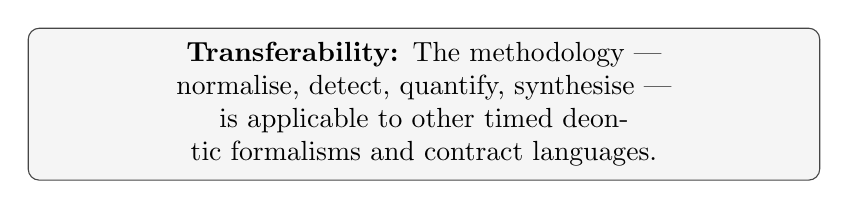
\begin{tikzpicture}
  \node[draw=ConflictGray,rounded corners,fill=gray!8,text width=0.8\textwidth,align=center,inner sep=5pt,font=\normalsize] {
  \textbf{Transferability:} The methodology \textemdash\ normalise, detect, quantify, synthesise \textemdash\\
  is applicable to other timed deontic formalisms and contract languages.
  };
\end{tikzpicture}

\vspace{4mm}
{\Large\bfseries Thank you! \quad Questions?}
\end{frame}

\begin{frame}{Backup Slides}
\begin{itemize}
  %hint look at \subsubsection{Syntax-Aware Conflict Detection: LUCO and LAP} in conflictmeat.tex
  \item Luco and LAP definition with intuitive explanation (pictures and formulas)
  %hint look after \begin{theorem}[Conflict-free rewriting]\label{thm:cfr} examples in conflictmea.tex
  \item examples of repair (positive and negative)
  %hin look for \caption{Conflict calculus for \TDDLfm} in conflictmeat.tex
  \item conflict calculus rules
  %hint look at \subsection{From Metric-Timed to Collaborative Periodic Synchronized Set Traces} in chaptermonitor.tex
  \item from Metric-Timed to Collaborative Periodic Synchronized Set Traces (the example in steps with arrow explanation)
  \item  
\end{itemize}

\end{frame}

\end{document}